\documentclass{standalone}
\usepackage{tikz}
\usepackage{tikz-3dplot}
\begin{document}


\tikzset{every picture/.style={line width=0.75pt}} %set default line width to 0.75pt        

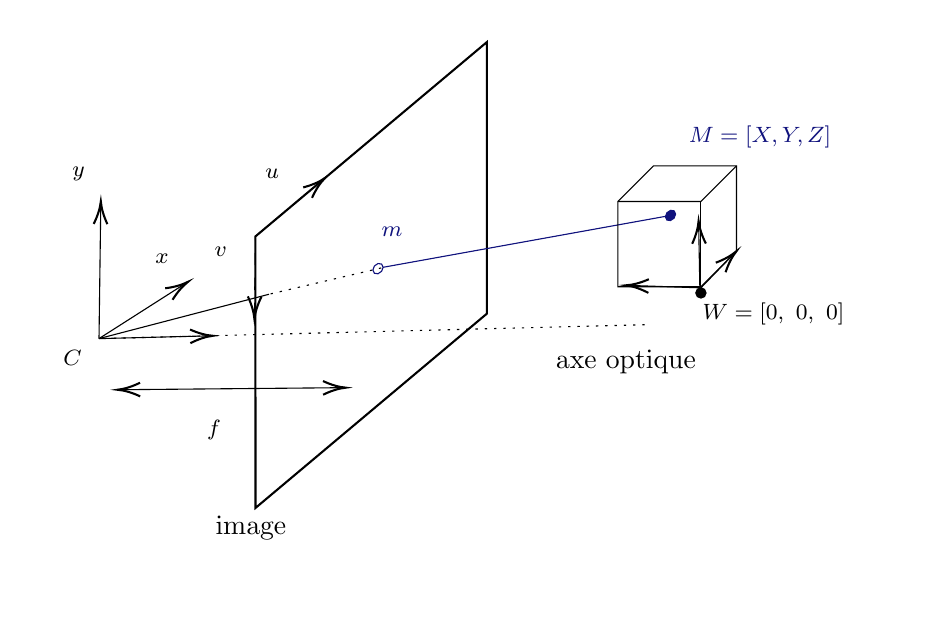
\begin{tikzpicture}[x=0.75pt,y=0.75pt,yscale=-1,xscale=1]
%uncomment if require: \path (0,300); %set diagram left start at 0, and has height of 300

%Shape: Rectangle [id:dp7601209230583179] 
\draw  [line width=0.75]  (261.98,12.03) -- (262.02,142.84) -- (150.52,236.47) -- (150.47,105.66) -- cycle ;
%Shape: Circle [id:dp6050690727269609] 
\draw  [color={rgb, 255:red, 16; green, 18; blue, 125 }  ,draw opacity=1 ][fill={rgb, 255:red, 16; green, 18; blue, 125 }  ,fill opacity=1 ] (350.47,93.07) .. controls (351.83,92.71) and (352.93,93.52) .. (352.93,94.88) .. controls (352.93,96.24) and (351.83,97.64) .. (350.47,98.01) .. controls (349.1,98.37) and (348,97.56) .. (348,96.2) .. controls (348,94.84) and (349.1,93.44) .. (350.47,93.07) -- cycle ;
%Shape: Circle [id:dp4188034345781906] 
\draw  [fill={rgb, 255:red, 0; green, 0; blue, 0 }  ,fill opacity=1 ] (365.12,130.42) .. controls (366.48,130.42) and (367.58,131.52) .. (367.58,132.88) .. controls (367.58,134.25) and (366.48,135.35) .. (365.12,135.35) .. controls (363.75,135.35) and (362.65,134.25) .. (362.65,132.88) .. controls (362.65,131.52) and (363.75,130.42) .. (365.12,130.42) -- cycle ;
%Straight Lines [id:da05981304354030248] 
\draw  [dash pattern={on 4.5pt off 4.5pt}]  (150.02,143.52) -- (150.47,105.66) ;
\draw [shift={(150,145.52)}, rotate = 270.68] [color={rgb, 255:red, 0; green, 0; blue, 0 }  ][line width=0.75]    (10.93,-3.29) .. controls (6.95,-1.4) and (3.31,-0.3) .. (0,0) .. controls (3.31,0.3) and (6.95,1.4) .. (10.93,3.29)   ;
%Straight Lines [id:da9349518610470805] 
\draw  [dash pattern={on 4.5pt off 4.5pt}]  (182.47,78.8) -- (150.47,105.66) ;
\draw [shift={(184,77.52)}, rotate = 139.99] [color={rgb, 255:red, 0; green, 0; blue, 0 }  ][line width=0.75]    (10.93,-3.29) .. controls (6.95,-1.4) and (3.31,-0.3) .. (0,0) .. controls (3.31,0.3) and (6.95,1.4) .. (10.93,3.29)   ;
%Shape: Circle [id:dp08218307241945377] 
\draw  [color={rgb, 255:red, 16; green, 18; blue, 125 }  ,draw opacity=1 ] (209.53,118.71) .. controls (210.9,118.35) and (212,119.15) .. (212,120.52) .. controls (212,121.88) and (210.9,123.28) .. (209.53,123.64) .. controls (208.17,124.01) and (207.07,123.2) .. (207.07,121.84) .. controls (207.07,120.48) and (208.17,119.08) .. (209.53,118.71) -- cycle ;
%Straight Lines [id:da6073826010308068] 
\draw [color={rgb, 255:red, 16; green, 18; blue, 125 }  ,draw opacity=1 ][fill={rgb, 255:red, 16; green, 18; blue, 125 }  ,fill opacity=1 ]   (350.47,95.54) -- (212,120.52) ;
%Straight Lines [id:da1040423634731219] 
\draw    (365.12,130.42) -- (331,129.27) ;
\draw [shift={(329,129.2)}, rotate = 1.93] [color={rgb, 255:red, 0; green, 0; blue, 0 }  ][line width=0.75]    (10.93,-3.29) .. controls (6.95,-1.4) and (3.31,-0.3) .. (0,0) .. controls (3.31,0.3) and (6.95,1.4) .. (10.93,3.29)   ;
%Straight Lines [id:da03925147237477766] 
\draw    (365.12,130.42) -- (380.86,114.19) ;
\draw [shift={(382.25,112.75)}, rotate = 134.12] [color={rgb, 255:red, 0; green, 0; blue, 0 }  ][line width=0.75]    (10.93,-3.29) .. controls (6.95,-1.4) and (3.31,-0.3) .. (0,0) .. controls (3.31,0.3) and (6.95,1.4) .. (10.93,3.29)   ;
%Straight Lines [id:da4025934746872343] 
\draw    (364.65,132.88) -- (364.04,100.2) ;
\draw [shift={(364,98.2)}, rotate = 88.93] [color={rgb, 255:red, 0; green, 0; blue, 0 }  ][line width=0.75]    (10.93,-3.29) .. controls (6.95,-1.4) and (3.31,-0.3) .. (0,0) .. controls (3.31,0.3) and (6.95,1.4) .. (10.93,3.29)   ;
%Shape: Cube [id:dp20886869978564915] 
\draw   (325.13,88.8) -- (342.27,71.67) -- (382.25,71.67) -- (382.25,112.75) -- (365.12,129.88) -- (325.13,129.88) -- cycle ; \draw   (382.25,71.67) -- (365.12,88.8) -- (325.13,88.8) ; \draw   (365.12,88.8) -- (365.12,129.88) ;
%Straight Lines [id:da39749877106333076] 
\draw [color={rgb, 255:red, 0; green, 0; blue, 0 }  ,draw opacity=1 ] [dash pattern={on 0.84pt off 2.51pt}]  (338,148.2) -- (75.12,154.88) ;
%Straight Lines [id:da17536155613259208] 
\draw [color={rgb, 255:red, 0; green, 0; blue, 0 }  ,draw opacity=1 ]   (75.12,154.88) -- (75.97,90.75) ;
\draw [shift={(76,88.75)}, rotate = 90.77] [color={rgb, 255:red, 0; green, 0; blue, 0 }  ,draw opacity=1 ][line width=0.75]    (10.93,-3.29) .. controls (6.95,-1.4) and (3.31,-0.3) .. (0,0) .. controls (3.31,0.3) and (6.95,1.4) .. (10.93,3.29)   ;
%Straight Lines [id:da14217393161245706] 
\draw [color={rgb, 255:red, 0; green, 0; blue, 0 }  ,draw opacity=1 ]   (75.12,154.88) -- (116.31,128.59) ;
\draw [shift={(118,127.52)}, rotate = 147.45] [color={rgb, 255:red, 0; green, 0; blue, 0 }  ,draw opacity=1 ][line width=0.75]    (10.93,-3.29) .. controls (6.95,-1.4) and (3.31,-0.3) .. (0,0) .. controls (3.31,0.3) and (6.95,1.4) .. (10.93,3.29)   ;
%Straight Lines [id:da32252527713710877] 
\draw [color={rgb, 255:red, 0; green, 0; blue, 0 }  ,draw opacity=1 ]   (75.12,154.88) -- (128,153.57) ;
\draw [shift={(130,153.52)}, rotate = 178.57] [color={rgb, 255:red, 0; green, 0; blue, 0 }  ,draw opacity=1 ][line width=0.75]    (10.93,-3.29) .. controls (6.95,-1.4) and (3.31,-0.3) .. (0,0) .. controls (3.31,0.3) and (6.95,1.4) .. (10.93,3.29)   ;
%Straight Lines [id:da7015838779144175] 
\draw [color={rgb, 255:red, 0; green, 0; blue, 0 }  ,draw opacity=1 ]   (157,133.52) -- (75.12,154.88) ;
%Straight Lines [id:da25429061987195445] 
\draw [color={rgb, 255:red, 0; green, 0; blue, 0 }  ,draw opacity=1 ]   (86,179.5) -- (192,178.53) ;
\draw [shift={(194,178.52)}, rotate = 179.48] [color={rgb, 255:red, 0; green, 0; blue, 0 }  ,draw opacity=1 ][line width=0.75]    (10.93,-3.29) .. controls (6.95,-1.4) and (3.31,-0.3) .. (0,0) .. controls (3.31,0.3) and (6.95,1.4) .. (10.93,3.29)   ;
\draw [shift={(84,179.52)}, rotate = 359.48] [color={rgb, 255:red, 0; green, 0; blue, 0 }  ,draw opacity=1 ][line width=0.75]    (10.93,-3.29) .. controls (6.95,-1.4) and (3.31,-0.3) .. (0,0) .. controls (3.31,0.3) and (6.95,1.4) .. (10.93,3.29)   ;

%Straight Lines [id:da3707521580726403] 
\draw [color={rgb, 255:red, 0; green, 0; blue, 0 }  ,draw opacity=1 ] [dash pattern={on 0.84pt off 2.51pt}]  (211.07,120.84) -- (157,133.52) ;


%Shape: Rectangle [id:dp5188287313383751] 
\draw  [color={rgb, 255:red, 255; green, 255; blue, 255 }  ,draw opacity=1 ] (41.02,5.34) -- (469,5.34) -- (469,280.34) -- (41.02,280.34) -- cycle ;

% Text Node
\draw (358,50.9) node [anchor=north west][inner sep=0.75pt]  [font=\footnotesize,color={rgb, 255:red, 16; green, 18; blue, 125 }  ,opacity=1 ]  {$M=[ X,Y,Z]$};
% Text Node
\draw (364.65,136.28) node [anchor=north west][inner sep=0.75pt]  [font=\footnotesize]  {$W=[ 0,\ 0,\ 0]$};
% Text Node
\draw (154,71.9) node [anchor=north west][inner sep=0.75pt]  [font=\footnotesize]  {$u$};
% Text Node
\draw (129.5,109.4) node [anchor=north west][inner sep=0.75pt]  [font=\footnotesize]  {$v$};
% Text Node
\draw (210,99.9) node [anchor=north west][inner sep=0.75pt]  [font=\footnotesize,color={rgb, 255:red, 167; green, 17; blue, 17 }  ,opacity=1 ]  {$\textcolor[rgb]{0.06,0.07,0.49}{m}$};
% Text Node
\draw (130,239) node [anchor=north west][inner sep=0.75pt]   [align=left] {image};
% Text Node
\draw (294,159) node [anchor=north west][inner sep=0.75pt]   [align=left] {axe optique};
% Text Node
\draw (56.65,159.28) node [anchor=north west][inner sep=0.75pt]  [font=\footnotesize]  {$C$};
% Text Node
\draw (61,70.9) node [anchor=north west][inner sep=0.75pt]  [font=\footnotesize]  {$y$};
% Text Node
\draw (101,112.9) node [anchor=north west][inner sep=0.75pt]  [font=\footnotesize]  {$x$};
% Text Node
\draw (126,192.9) node [anchor=north west][inner sep=0.75pt]  [font=\footnotesize]  {$f$};


\end{tikzpicture}
\end{document}
